% #############################################################################
% model_overview.tex
% Irrigation Technology Adoption Replicator-Dynamics Model
% Author: Yoshi Budiyanto, Arizona State University
% #############################################################################
\documentclass[10pt,border=0pt]{standalone}
\usepackage{graphicx,tikz,setspace}
\usepackage[nopatch={eqnum,footnote}]{microtype}
\microtypesetup{expansion=false}
\DisableLigatures[f]{encoding = *, family = * }
\usetikzlibrary{arrows.meta,positioning,calc}
\definecolor{modelblue}{HTML}{1F4E79}
\definecolor{modelbluefill}{HTML}{EAF2F8}
\definecolor{levergreen}{HTML}{2A7F62}
\definecolor{levergreenfill}{HTML}{E8F5EE}
\doublespacing
\setlength{\textwidth}{5.25in}
\begin{document}
\begingroup
\setstretch{1}
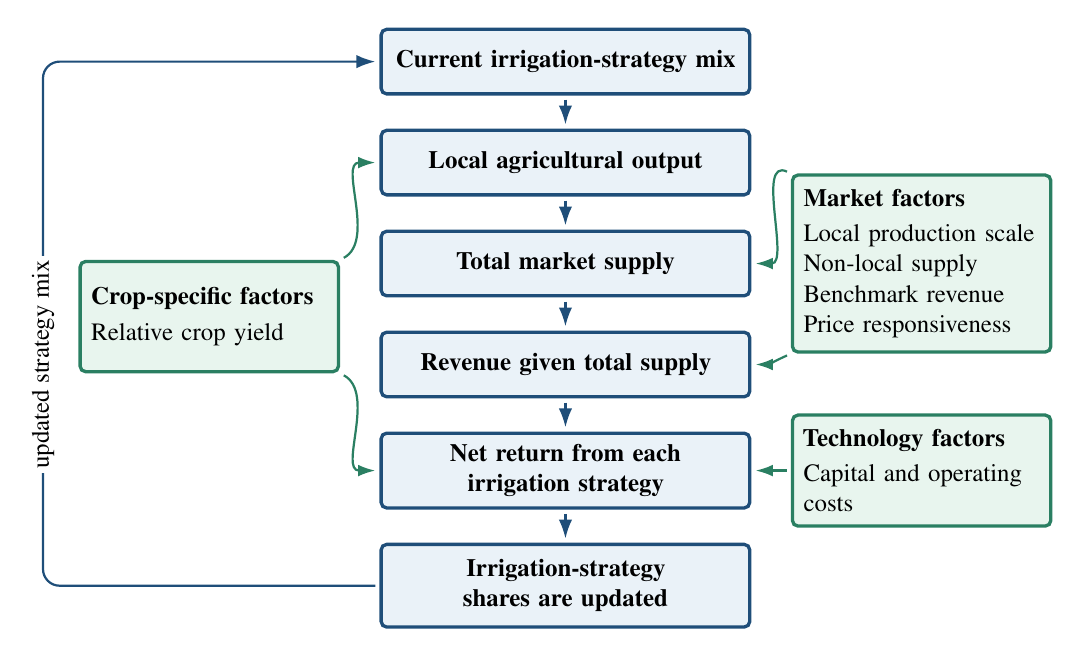
\begin{tikzpicture}[
  font=\fontfamily{ptm}\fontsize{9}{11}\selectfont,
  core/.style={
    rounded corners=2pt,
    draw=modelblue,
    very thick,
    fill=modelbluefill,
    align=center,
    text width=4.40cm,
    minimum height=0.82cm,
    inner xsep=4pt,
    inner ysep=4pt
  },
  lever/.style={
    rounded corners=2pt,
    draw=levergreen,
    very thick,
    fill=levergreenfill,
    align=left,
    text width=3.00cm,
    minimum height=1.05cm,
    inner xsep=4pt,
    inner ysep=5pt
  },
  flow/.style={
    -{Latex[length=2.4mm,width=1.7mm]},
    thick,
    draw=modelblue,
    shorten <=1.5pt,
    shorten >=1.5pt
  },
  input/.style={
    -{Latex[length=2.2mm,width=1.5mm]},
    thick,
    draw=levergreen,
    shorten <=1.5pt,
    shorten >=1.5pt
  },
  feedback/.style={
    -{Latex[length=2.4mm,width=1.7mm]},
    thick,
    draw=modelblue,
    shorten <=1.5pt,
    shorten >=1.5pt
  }
]


\node[core] (shares)
  {
    \textbf{Current irrigation-strategy mix}
  };

\node[core, below=0.42cm of shares] (output)
  {
    \textbf{Local agricultural output}
  };

\node[core, below=0.42cm of output] (supply)
  {
    \textbf{Total market supply}
  };

\node[core, below=0.42cm of supply] (revenue)
  {
    \textbf{Revenue given total supply}
  };

\node[core, below=0.42cm of revenue] (payoff)
  {
    \textbf{Net return from each irrigation strategy}
  };

\node[
  core,
  minimum height=1.05cm,
  below=0.42cm of payoff
] (update)
  {
    \textbf{Irrigation-strategy shares are updated}
  };


\coordinate (cropmid)
  at ($(output.west)!0.5!(payoff.west)$);

\node[
  lever,
  anchor=east,
  minimum height=1.40cm
] (crop)
  at ($(cropmid)+(-0.50cm,0)$)
  {
    \textbf{Crop-specific factors}\\[0.20em]
    Relative crop yield
  };


\coordinate (marketmid)
  at ($(supply.east)!0!(revenue.east)$);

\node[
  lever,
  anchor=west,
  minimum height=2.05cm
] (market)
  at ($(marketmid)+(0.50cm,0)$)
  {
    \textbf{Market factors}\\[0.20em]
    Local production scale\\
    Non-local supply\\
    Benchmark revenue\\
    Price responsiveness
  };


\node[
  lever,
  anchor=west,
  minimum height=1.40cm
] (technology)
  at ($(payoff.east)+(0.50cm,0)$)
  {
    \textbf{Technology factors}\\[0.20em]
    Capital and operating costs
  };


\draw[flow]
  (shares.south) -- (output.north);

\draw[flow]
  (output.south) -- (supply.north);

\draw[flow]
  (supply.south) -- (revenue.north);

\draw[flow]
  (revenue.south) -- (payoff.north);

\draw[flow]
  (payoff.south) -- (update.north);


\draw[input]
  (crop.north east)
  to[out=28,in=180]
  (output.west);

\draw[input]
  (crop.south east)
  to[out=-28,in=180]
  (payoff.west);


\draw[input]
  (market.north west)
  to[out=155,in=0]
  (supply.east);

\draw[input]
  (market.south west)
  to[out=-155,in=0]
  (revenue.east);


\draw[input]
  (technology.west) -- (payoff.east);


\coordinate (feedbackx)
  at ($(crop.west)+(-0.45cm,0)$);

\draw[
  feedback,
  rounded corners=6pt
]
  (update.west)
  -- (feedbackx |- update.west)
  -- (feedbackx |- shares.west)
  -- (shares.west);

\node[
  rotate=90,
  fill=white,
  inner sep=1.5pt
] at ($(feedbackx |- revenue.west)$)
  {updated strategy mix};

\end{tikzpicture}
\endgroup
\end{document}
